\documentclass[margin,line]{res}
\usepackage{hyperref}
\usepackage{url}
\oddsidemargin -.5in
\evensidemargin -.5in
\textwidth=6.0in
\itemsep=0in
\parsep=0in
\topmargin=0in
\topskip=0in
\usepackage{graphicx}
\newenvironment{list1}{
  \begin{list}{\ding{113}}{%
      \setlength{\itemsep}{0in}
      \setlength{\parsep}{0in} \setlength{\parskip}{0in}
      \setlength{\topsep}{0in} \setlength{\partopsep}{0in}
      \setlength{\leftmargin}{0.17in}}}{\end{list}}
\newenvironment{list2}{
  \begin{list}{$\bullet$}{%
      \setlength{\itemsep}{0in}
      \setlength{\parsep}{0in} \setlength{\parskip}{0in}
      \setlength{\topsep}{0in} \setlength{\partopsep}{0in}
      \setlength{\leftmargin}{0.2in}}}{\end{list}}


    
\begin{document}

\name{\LARGE Bharath.T.U} \hfill {\em \today}

\begin{resume}
\section{\sc Contact Information}

\vspace{.05in}
\begin{tabular}{@{}p{3.5in}p{3in}}
2nd  Year B.Tech Student                                                                     & {Phone:}  9497531920 \\
Mar Baselios College Of Engineering
and Technology 
 & {E-mail:}  bharath218usba@gmail.com\\
Mar Ivanios College Rd, Nalanchira.\\
Thattinakam, Thiruvananthapuram, Kerala 695015.\\ 
&
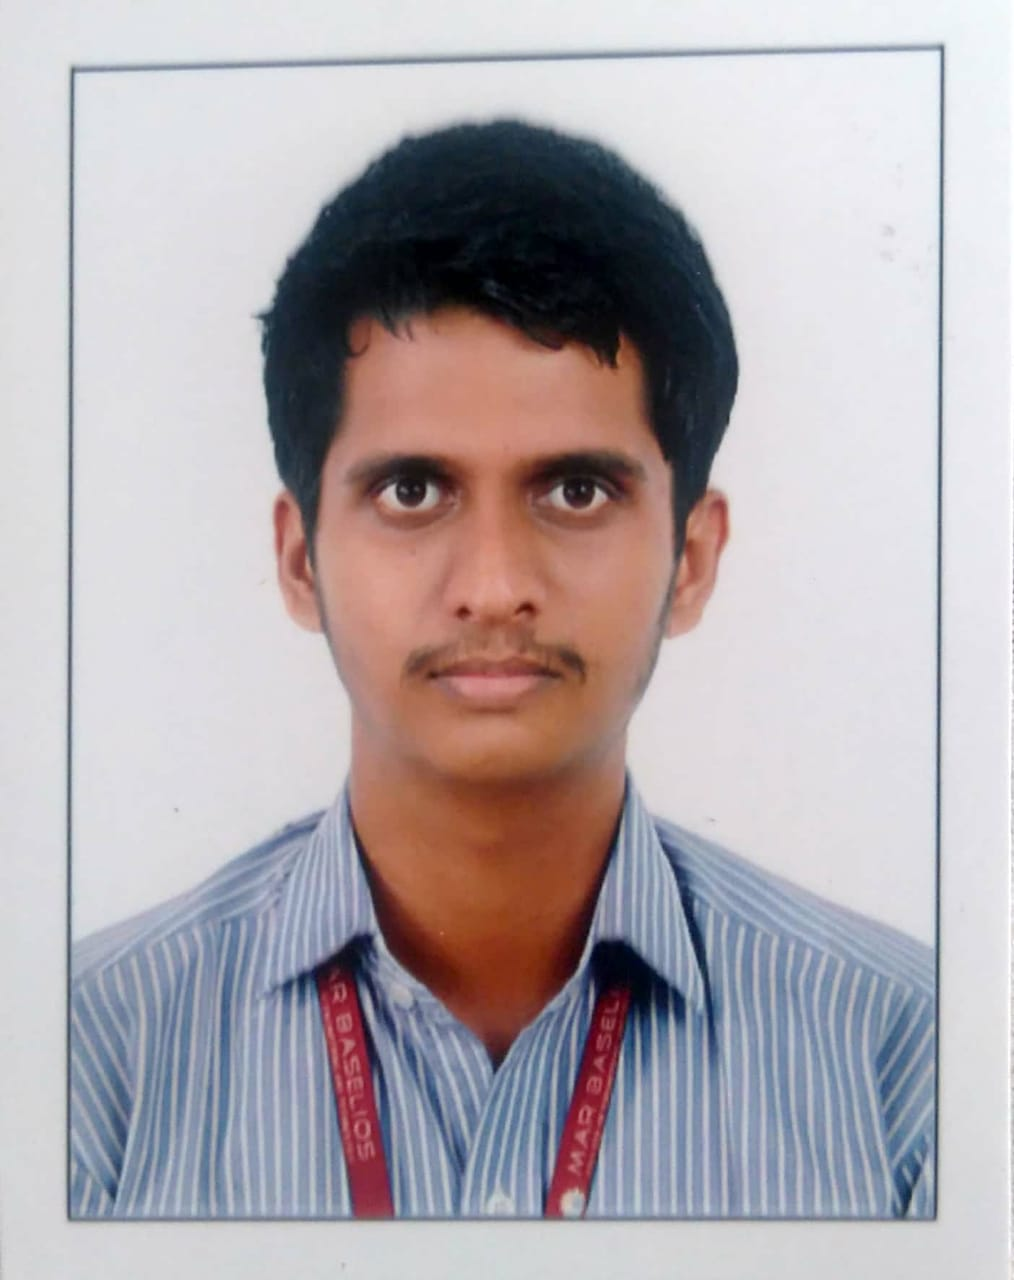
\includegraphics[width=0.1\textheight]{bh}

\end{tabular}

\vspace{.1in}
\section{\sc OBJECTIVE}

To be relevant on the new technologies and have a research or Innovation based career in the field of machine learning , robotics , Iot and networking
\vspace{.1in}
\section{\sc Education}
\begin{tabular}{|l|c|l|c|l|c|}\hline
	\bf Degree&\bf College/School&\bf University&\bf Passing Year&\bf Pass Percentage \\ \hline
	BTech in CSE
	&MBCET & KTU & 2017-Present&1st 2 sem CGPA = 7.68/10 \\ \hline
	Class XII
	&KV-PANGODE & CBSE-AISSCE  & 2017& Overall = 84 Percentage \\&&&&99 Percentage in CS 
	
	\\ \hline
	Class X
	&KV-PANGODE & CBSE-AISSCE  & 2017& Overall = 81.7 Percentage 
	
	\\ \hline
\end{tabular}
\section{\sc PROJECTS}

\begin{enumerate} %Job Description%
	\item omni-directional wheel design \\
	\item Basic implementation of home automation\\
	\item Wireless basket ball count down timer display\\
\end{enumerate}

\section{\sc Training and Internship}
Trained in arduino \\
\section{\sc Research and Publication}

\bf NIL
\vspace{.1in}
\section{\sc Technical Skills}
{\bf Programming and Scripting Languages}:  C, Cpp,Python,Beginner at java \\
{\bf Operating Systems}: Windows and Beginner at Linux,\\
{\bf Database Tools}  :  Beginner at MySql\\
{\bf Software Pakages}:  Beginner at opencv\\

%%%%%%%%%%%%%%%%%%%
\section{\sc Soft Skills}
\begin{enumerate} %Job Description%
	\item Leadership 
	\item Colabration and Teamwork
	\item Strong work ethic 
	\item learnability 
	\item Creative thinking
\end{enumerate}
%%%%%%%%%%%%%%%%%%%
\section{\sc Extra-Curricular Activities}
\begin{list2} %Job Description%
	\item \bf School Of AI  \\
	Actively Participating meetups conducted by School of AI Thrivandrum
	
\end{list2}

%%%%%%%%%%%%%%%%%%%
\section{\sc Co-Curricular Activities}
\begin{enumerate} %Job Description%
	\item \bf EYRC 2018-19 \\
	1st runnerup in the theme HOMECOMING in e-Yantra IIT ROBOTICs competition \\
	\item \bf Mission Reconnect-2018\\
	Volunteered for Mission Reconnect-2018 by KSEB \\
	\item \bf LCD DISPLAY   \\
	Volunteered for LCD DISPLAY for our college (MBCET) \\
	\item Game of codes 2017 (python coding compition) 1st position\\
	\item Roborace IEDC catalyst 1st runner-up\\
	\item Roborace Cult A Way 2nd runner-up \\
	
\end{enumerate}
%%%%%%%%%%%%%%%%%%%
%%%%%%%%%%%%%%%%%%%
\section{\sc Professional Experience}
%%%%%%
{\bf MBCET}, TVM, KERALA. INDIA. \hfill{August 2017 -- Present}\\
\\

{\em Executive Member  OF DSC }\hfill {Feburary 2019 -- Present}\\
\begin{list2} %Job Description%
	\item Responsible for Spreading awarness about DSC  \\
	\item Coordinating DSC retated activities.
\end{list2}
{\em Executive Member  OF OPENLABs }\hfill {Feburary 2019 -- Present}\\
\begin{list2} %Job Description%
	\item Responsible for Technical team  \\
	
\end{list2}
%%%%%%%%%%%
%%%%%%%%%%%%%%%%
\section{\sc Personal Details}
{\bf Father's Name}: Unnikrishnan.T.N \\
{\bf Mothers's Name}:  Sunita S\\
{\bf Sex}  :  MALE\\
{\bf Date Of Birth}:  21th August 2000\\
{\bf Nationality}       : Indian \\
{\bf Marital Status}       : Single \\



\section{\sc REFERENCE }

\bf Tessy Mathew ,\\ Head of Department of Computer Science and Engineering, Mar Baselios College Of Engineering and Technology, +91 9447696899, Tessy.mathew@mbcet.ac.in


\bf Arun J S,\\ Mentors at K-DISC and
Professor at Department of Electronics and Communication\\ of Engineering, Mar Baselios College Of Engineering andTechnology, +91 9496368197, mearunjs@gmail.com
\section{\sc DECLARATION}
I do hereby declare that above particulars of information and facts stated are true, correct and complete to the best of my knowledge and belief.
\end{resume}
\end{document}


